\section{Architecture}

The CoVidA application architecture is structured as shown in Figure \ref{fig:uml}.
All core functionallities are bundled in the covida-core package.
All visual components are handled from the visual package, which is exchangeable.
In this setup the covida-visual-jme2 package is used to render the covida application.
The video package is also exchangeable and currently is the covida-video-vlcj package used which has the vlcj as foundation.

\begin{figure}[!ht]
\captionsetup{type=figure} 
 \centering
 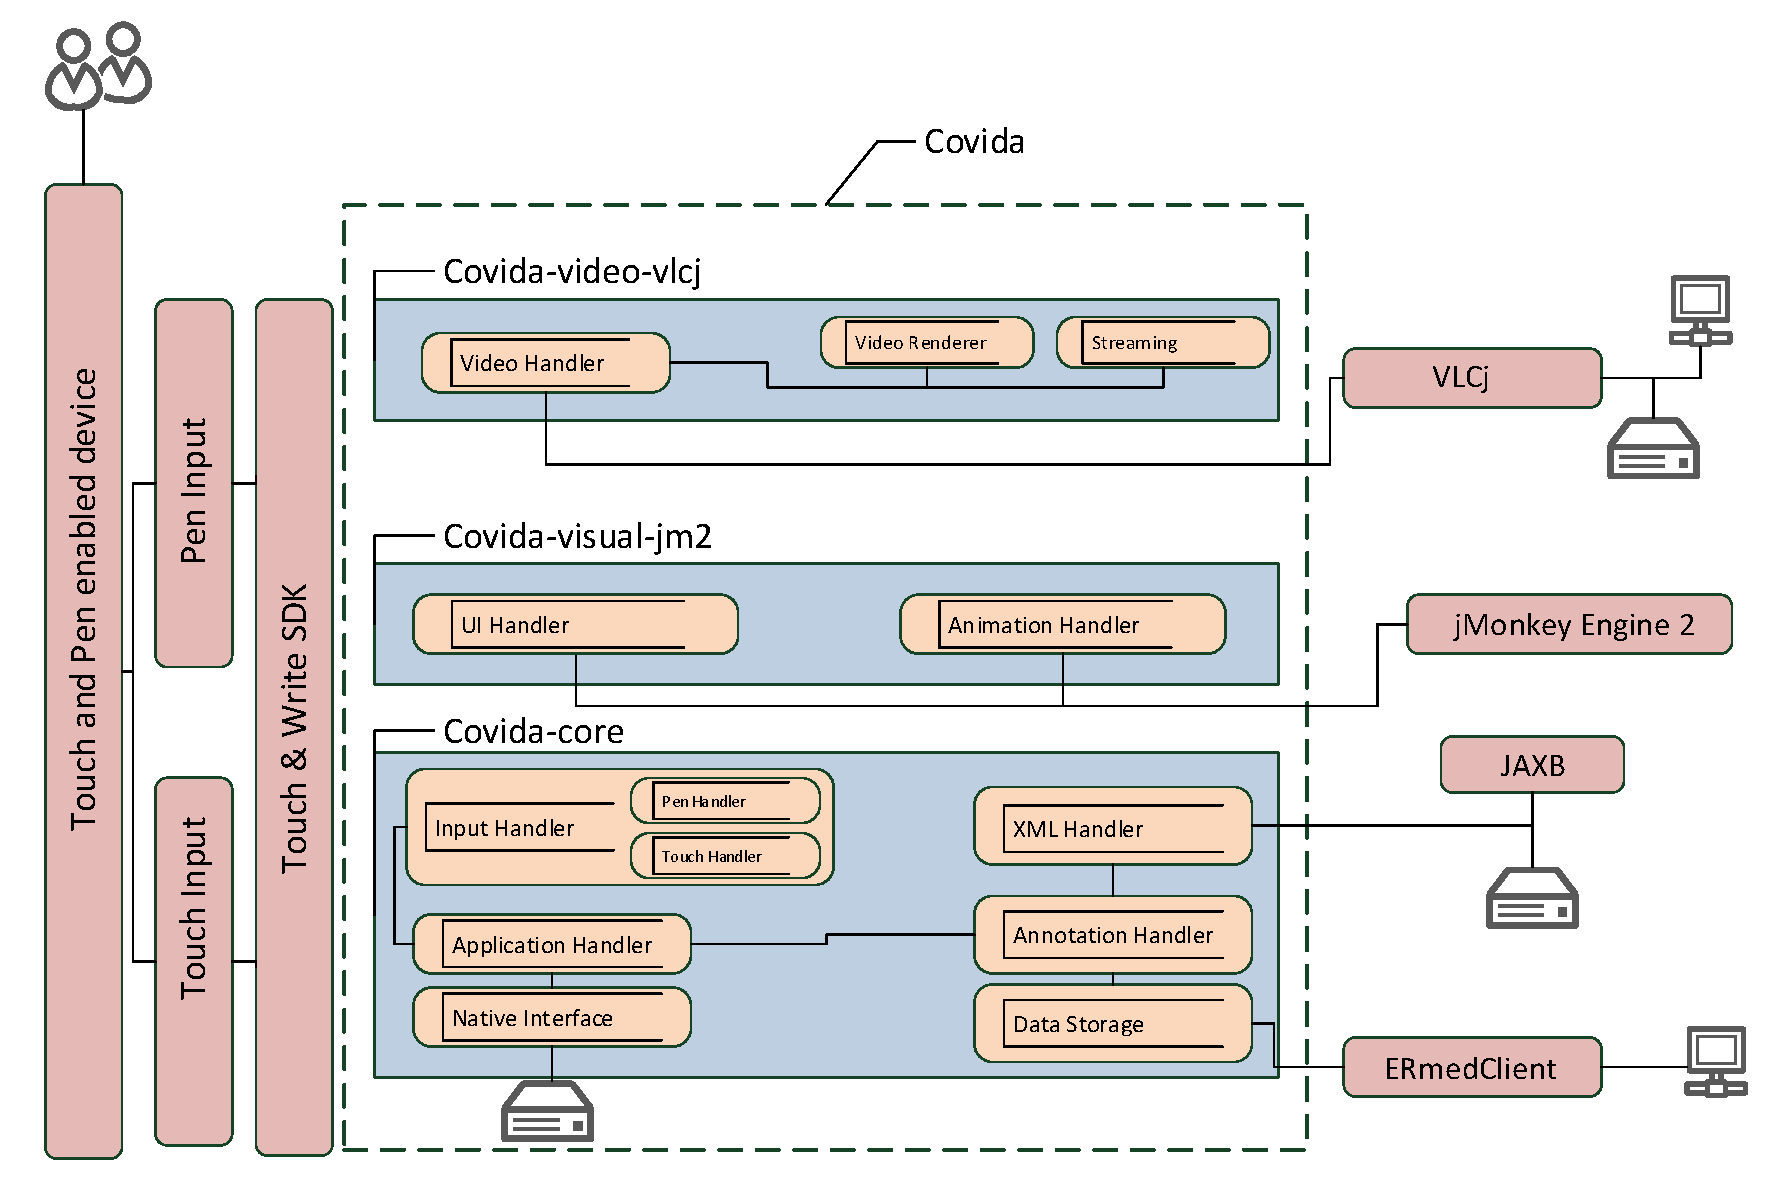
\includegraphics[width=.85\columnwidth]{architecture}
 \caption{Covida Architecture.}
 \label{fig:uml}
\end{figure}

In the current setup (Figure \ref{fig:uml}) three third party components are used.
First the TouchAndWrite SDK which is used as basis for the covidacore component.
Second the VLCj component which provides the videovlcj component whith methods to handle a huge variaty of video formats.
Finally the jMonkey Engine 2 (jme2) is a scene graph based 3D engine framework completly
written in Java2. The CoVidA presentation layer gives with aid of the jMonkey Engine 2
framwork graphical feedback onto user interactions. With this framework CoVidA has the
possibility to move and transform multiple videos and switch textures directly. For other
feedback, like opening or closing, the jMonkey Engine 2 offers CoVidA the possibility
to animate the user interface objects and control this animations in case they must be
interupted.